\documentclass[11pt]{article}
\usepackage[margin=0.82in]{geometry}
\usepackage{booktabs, longtable, array, graphicx, amsmath, xcolor, hyperref, xurl}
\usepackage[authoryear,round]{natbib}
\hypersetup{colorlinks=true, urlcolor=blue, linkcolor=blue, citecolor=blue}
\renewcommand{\arraystretch}{1.25}
\setlength{\emergencystretch}{1em}
\setlength{\parskip}{5pt}\setlength{\parindent}{0pt}
\title{Simplifying assumptions in power analysis:\\A replication of Kupzyk (2011)}
\date{29 October 2026}
\begin{document}\maketitle\vspace{-2em}
\begin{abstract}
We replicated the final-stage exemplary-data headline of \citet{kupzyk2011}: attrition and unequal treatment allocation reduce power more than the tested unequal cluster sizes (published versus reconstructed losses: 1.327 versus 1.275, 4.391 versus 4.476, 6.409 versus 6.446, and 0.652 versus 0.609 percentage points, respectively). All four differences lie within two standard deviations of the source's single-dropout-mask variation; none is separated after Holm adjustment. We could not establish an exact replay of SAS or the original random masks, and the reported minimum cluster counts are not uniquely recoverable across masks. The empirical baseline agrees with the published empirical value (.86712 versus 0.86675), but remains below the fixed-variance exemplary result (0.86675 versus 0.87721); this gap survives Holm correction across 54 cells, and the paired variance-estimation diagnostic provides evidence against explaining that gap solely as Monte Carlo noise.
\end{abstract}
\begin{center}\small
\begin{tabular}{p{.25\linewidth}rrrr}
\toprule Claim (loss, percentage points)&Published&Ours&Direction&Verdict\\\midrule
5\% interval attrition&1.327&1.275&Yes&match\\
15\% interval attrition&4.391&4.476&Yes&match\\
70/30 allocation&6.409&6.446&Yes&match\\
Unequal cluster sizes&0.652&0.609&Yes&match\\
\bottomrule\end{tabular}
\end{center}
{\footnotesize Tolerance: two predictive standard deviations for a contrast of the original single-mask cells, followed by Holm correction over these four contrasts. This is not a confidence interval for our simulated mean. Published losses are calculated from Table~1's printed cells \citep[p.~92]{kupzyk2011}, retaining more precision than the rounded prose.}
\section{What replicated?}
We replicated the four final exemplary power losses:1.327/1.275,4.391/4.476,6.409/6.446, and 0.652/0.609 percentage points (published/ours), within the stated mask-aware tolerance. Exact original software and random streams remain unverified. The empirical-versus-exemplary difference is examined separately below, rather than treating the fixed-variance calculation as empirical power.

Kupzyk reports these final-stage conclusions on pp.~93--96 \citep{kupzyk2011}. The research question is whether ignoring dropout, unequal treatment allocation, or unequal cluster sizes misstates the power of a longitudinal cluster randomized trial. Kevin A. Kupzyk's April 2011 University of Nebraska--Lincoln dissertation, \emph{The Effects of Simplifying Assumptions in Power Analysis}, names Professor James A. Bovaird as supervisor on PDF page 2 and as adviser in the abstract. The \href{https://digitalcommons.unl.edu/cehsdiss/106/}{official repository record} independently confirms the adviser. This is a new dissertation relative to the Abbott and Chumney replications.

All 18 no-attrition Table 1 values round to the published five decimal places. The 36 attrition cells depend on random dropout ranks, even in the exemplary-data code. Comparing their single published realizations with our means at five decimals yields mostly numerical mismatches; those labels are retained in the detailed table and do not establish a substantive failure. Two cells fall beyond two predictive standard deviations before multiplicity correction (cells 9 and 35); no cell remains separated after Holm correction. These are tests of compatibility with the reconstructed mask distribution, not proof that a particular original mask was recovered.

The loss associated with 15\% interval attrition is greatest at ICC .05 and smaller at .10 and .15. Here ICC refers to the fraction of slope variance attributable to clusters, not the correlation of the raw outcome at an arbitrary wave. The result is conditional on the tested design: four waves, mean 20 participants per cluster, and treatment effect .5.
\begin{figure}[ht]\centering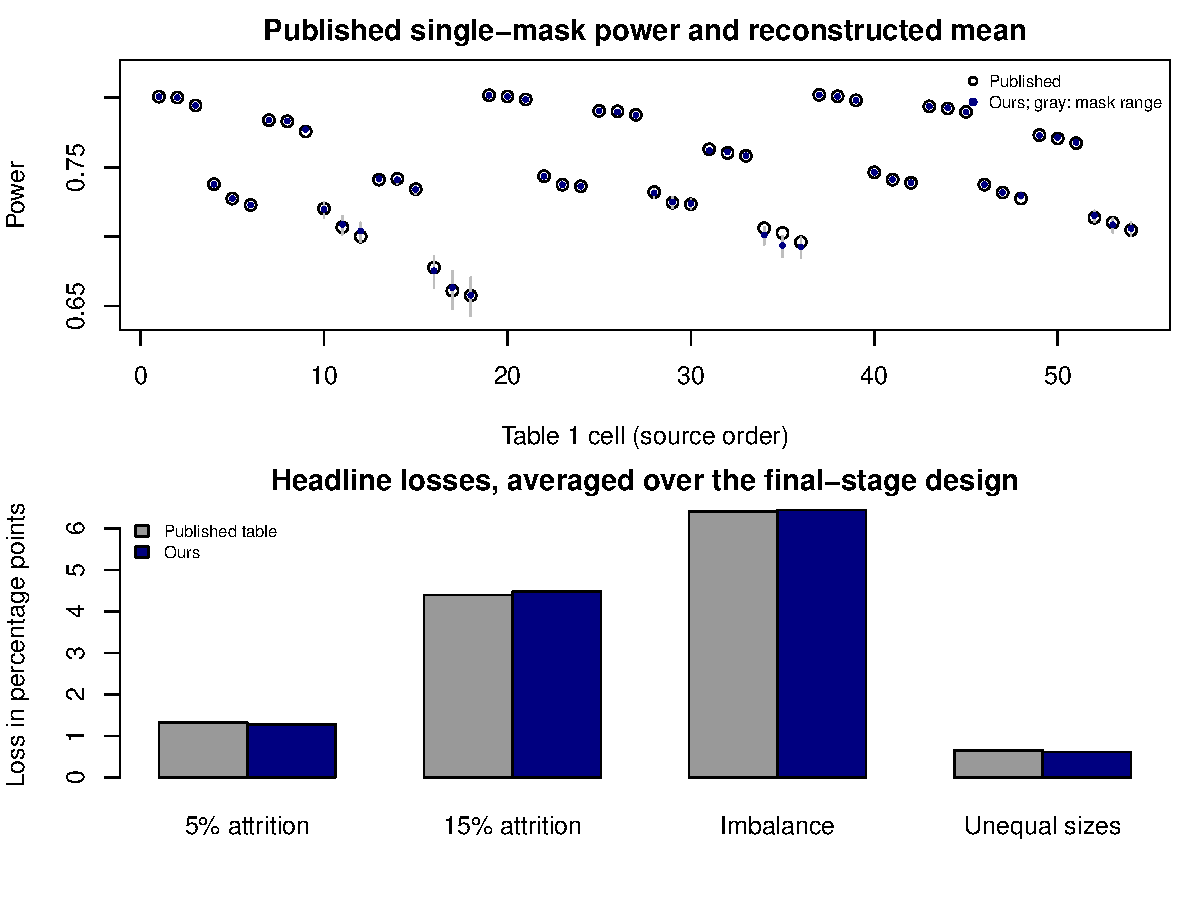
\includegraphics[width=.94\linewidth]{comparison-plot.pdf}\caption{Our calculations compared with published Table 1 \citep[p.~92]{kupzyk2011}. Gray ranges show empirical 2.5th--97.5th percentiles across new dropout masks; they are predictive ranges, not confidence intervals for the mean.}\end{figure}
\section{What did we calculate, and what came from the dissertation?}
The dissertation supplies the design and population model (pp.~79--90), printed SAS programs (Appendices A/B, pp.~124--129), and target tables (pp.~92--97) \citep{kupzyk2011}. Our contribution is the R translation, independently coded covariance calculation, new Monte Carlo draws, numerical comparisons, and sensitivity checks. No original participant data are involved: the study is a synthetic-data simulation. Original seeds, saved masks, and fitted output are not available in the materials obtained.

The exemplary-data approach also has a methodological history. Kupzyk credits \citet{obrien1993} for the terminology and \citet{stroup2002} for mixed-model power calculations \citep[pp.~53--56]{kupzyk2011}. Here the attribution to those detailed procedures is through Kupzyk: we verified the chapter's bibliographic record in the official SAS bibliography and Stroup's publisher metadata and abstract, but did not obtain either full text. Consequently, Appendix B remains the directly inspected specification for our implementation, rather than an inferred reconstruction of those earlier works.

We distinguish the initial stage, with 16,22,28 clusters at ICC .05,.10,.15, from the final stage, with 13,19,25. The 54 final cells cross three ICCs, three attrition rates, two treatment allocations, and three cluster-size distributions. Every final exemplary cell was run. Every initial empirical cell was run at reduced scale. Formulaic OD and BW variants, oversampling, and reported cluster thresholds were also evaluated.

We derive the following covariance from the independent random components in Kupzyk's Appendix A \citep[pp.~124--126]{kupzyk2011}; this matrix expression is our reconstruction. For observed outcome rows within one cluster, our covariance matrix is
\[
 V_{ab}=.1+\rho t_a t_b+I(i_a=i_b)\{.2+(1-\rho)t_at_b\}+.5I(a=b).
\]
With fixed-effect matrix $X=[1, t, g, tg]$, the interaction variance is the fourth diagonal element of $(\sum_j X_j'V_j^{-1}X_j)^{-1}$. The exemplary noncentrality is $.25/\operatorname{Var}(\widehat\beta_{tg})$. Power is the upper tail of a noncentral F distribution at the central .95 quantile, with numerator df 1. This directly translates Appendix B's held variance components and noncentral-F calculation \citep[pp.~127--129]{kupzyk2011}; it does not fit noise-free outcomes to estimate residual variance.

The formulaic arms also reproduce the direction and approximate magnitude of the source's df effect: at 16 clusters and ICC .05, our OD-rule power is .82731 and BW-rule power is .87721. The formula's equal allocation treats odd cluster counts continuously; actual exemplary data must allocate an integer number to each arm. Longitudinal power depends on the precision of the estimated rate of change; \citet{raudenbush2001} develop this connection for group differences in polynomial change. Their two-level complete-data model is background, not an exact statement of this three-level dropout design. In our reconstruction, the longitudinal formula includes the slope measurement-error term .5 divided by the sum of squared centered times (5), giving .1. It is not the cross-sectional Equation 2.22 used unchanged. This explains the small difference between a continuous-allocation formula and the final 13-cluster baseline without changing the model.

One implementation constructs each full cluster covariance and uses Cholesky solves. A second reduces each person's observed waves to a 2-by-2 information matrix and applies the Woodbury identity for cluster effects. Across 54 conditions the maximum absolute interaction-variance difference was 0.00000000000000. These independently coded calculations validate numerical assembly, not the missing SAS execution.
\section{Which assumptions did we supply?}
\subsection{Degrees of freedom with missing or unequal observations}
The source states $JnT-J-2$ for complete equal clusters and reports 1262 for $J=16, n=20, T=4$ \citep[Eq.~4.1, pp.~85--86]{kupzyk2011}. SAS describes the between/within partition \citep[MODEL statement, DDFM=BETWITHIN]{sasbw}, but that description alone does not establish our missing-data extension. We generalize this as $M-J-2$, where $M$ is the number of usable outcome rows. This follows the rank of cluster indicators plus the two within-cluster columns $t$ and $tg$; explicit rank checks pass in all 54 conditions. It is a source-consistent derived rule, not a verified output fixture from SAS. We also calculate power using $J-2$, $M-N-2$, and nominal $80J-J-2$, keeping the covariance fixed to isolate the reference distribution.
\subsection{Random streams and uncertainty}
New documented R seeds replace the unspecified SAS rannor(0)/ranuni(0) streams. The final exemplary run uses 1000 independent masks in each attrition cell and one exact calculation without attrition. Original cells are treated as independent mask realizations when computing predictive contrast variation; their actual random-stream dependence is unrecorded. Our mean standard errors are reported separately. Original single-mask variation is not divided by 1000. Monte Carlo rejection rates use two binomial standard errors; reporting simulation precision separately from the estimated performance follows \citet{morris2019}. Comparisons across 54 cells receive Holm's sequential correction \citep{holm1979}. Our two-predictive-SD compatibility band for random masks is a study-specific choice, not a rule prescribed by either reference.
\subsection{Failure and boundary policy}
Zero variance estimates remain in the analysis. We report boundary fits separately from failed optimization, retry genuine convergence problems using nloptwrap, and report failures remaining after the retry. Conditional rejection rates exclude unresolved failures, while unconditional lower/upper bounds treat every failed fit as a nonrejection/rejection. This avoids silently interpreting a missing SAS numeric p-value as a significant result.
\subsection{Computational subset}
The pilot covered all 54 cells and averaged 0.0963 seconds per fit. The declared budget uses 400 empirical draws per cell,12000 total at the first baseline,2000 null draws at each extreme cell, and 200 independent-generator draws in four corner cells. Three single-thread workers preserve memory and CPU headroom, and 100-draw checkpoints support resumption. These are new reduced runs, not the dissertation's full 25,600-per-cell simulation. The source's planned 26,000 versus executed 25,600 is documented, not silently resolved. A 400-draw cell at power .8 has a two-SE band of about 4 percentage points and cannot resolve a 1-percentage-point gap reliably.
\section{What explains differences between empirical and exemplary power?}
The baseline comparison tests the idea that only Monte Carlo noise separates the methods. Our baseline empirical power was 0.86675 with SE 0.00310, versus exemplary 0.87721. The gap was -1.046 percentage points (-3.37 empirical standard errors). The source reports a 1.1-point initial gap and a 0.9-point gap after 50,000 draws, rather than a precise original first-cell power table in the results narrative \citep[pp.~85--90]{kupzyk2011}.

The source's Appendix D also reports baseline BW empirical power .86712 and OD empirical power .82416 \citep[Appendix D]{kupzyk2011}. These are empirical targets, distinct from the fixed-variance result .87721. Our saved baseline outputs permit direct comparison of both reference distributions and of known versus refitted variance on the same coefficient draws. Original exact run counts for each Appendix D row are not separately supplied, so source Monte Carlo precision should not be invented.

A simple independent cluster-slope calculation predicts .86920 when a noncentral t distribution with 14 degrees of freedom is compared with the BW critical value, versus .87721 for the fixed-variance exemplary calculation. This diagnostic isolates variance estimation: the sampling distribution changes when the denominator is estimated. It approximates the full variance-component model and is not labeled an exact procedure replay. It shows why equality of the two methods is not guaranteed merely by increasing the number of draws.

Across our full empirical exercise, 38000 fits were requested and 0 remained failed after retries; 1767 had a reported boundary solution. Per-cell counts, binomial bands, and unconditional bounds are in \href{https://github.com/alectionary/vibe-math/blob/master/formalization/kupzyk-power-assumptions/outputs/empirical-summary.csv}{empirical-summary.csv}. The independent dense-covariance generator is checked on four corner conditions; it creates a multivariate Gaussian draw directly instead of summing random effects. These two construction paths have the same intended Gaussian covariance but different code and streams.

Sixty shared datasets were fitted with both lme4 \citep{bates2015} and nlme \citep{nlme2025} REML, with all 60 converging in each engine. The maximum absolute coefficient difference was 0.00000223, and the maximum standard-error difference was 0.00001967. A second lme4 optimizer agrees similarly. Replacing REML with ML can move a shared-dataset p-value by as much as 0.0304; it is therefore not an interchangeable default. Official SAS documentation identifies REML as the PROC MIXED default \citep[METHOD option]{sasreml}.

On the same baseline coefficient draws, using the known population variance rejects in 0.88050 of draws, while re-estimating variance rejects in 0.86675. The paired difference is -1.375 percentage points with paired standard error 0.221. This direct same-draw diagnostic is more precise than contrasting two independent simulation runs. It supports a variance-estimation mechanism without claiming an exact distribution for the full restricted-variance-component fit. See \href{https://github.com/alectionary/vibe-math/blob/master/formalization/kupzyk-power-assumptions/outputs/baseline-diagnostic.csv}{baseline-diagnostic.csv}.

The null experiments compare BW with $J-2$ on the same fitted statistics. Supporting Satterthwaite calculations use 20 draws per endpoint/effect condition, with a 5-draw Kenward--Roger subset per condition because dense corrections cost more. The implemented Satterthwaite and Kenward--Roger diagnostics are described by \citet{kuznetsova2017} and \citet{halekoh2014}, respectively. Those small diagnostics verify implementation and reference-distribution sensitivity, not precise Type I error rates. Their exact counts and timings are supplied in \href{https://github.com/alectionary/vibe-math/blob/master/formalization/kupzyk-power-assumptions/outputs/df-diagnostics.csv}{df-diagnostics.csv}; neither method silently replaces BW.
\section{Which ambiguities were resolved?}
\subsection{Dropout is cumulative and globally ranked}
Appendices A/B remove exactly rounded $aN$, $2aN$, and $3aN$ persons at later waves, using the original total $N$ and one global rank per person. Thus 15\% interval dropout ends with 45\% dropout, not multiplicative survival. Earlier observed waves remain. The executable check in \href{https://github.com/alectionary/vibe-math/blob/master/formalization/kupzyk-power-assumptions/scripts/verify_engines.R}{verify\_engines.R} records expected row counts and rank-derived df in \href{https://github.com/alectionary/vibe-math/blob/master/formalization/kupzyk-power-assumptions/outputs/design-checks.csv}{design-checks.csv}. Reproduce with the README command at pinned repository base dbbdda83\allowbreak{}d1acce5d\allowbreak{}dd86e9ab\allowbreak{}7c27d79f\allowbreak{}2f300e12.
\subsection{Cluster sizes and half-up rounding}
Appendix B's 29 printed frequency rows are extracted directly from Library text and checked to total 13 through 41 clusters. Alternating placement between vector halves preserves treatment ordering. SAS positive half-up rounding is implemented explicitly; R's default ties-to-even would change odd-cluster allocation. Empirical skewed sizes follow the source's alternating transform of above 20 draws, rather than a generic skew-normal distribution. The exact arrays and parser are included; key implementations are \href{https://github.com/alectionary/vibe-math/blob/master/formalization/kupzyk-power-assumptions/scripts/model.R#L6}{cluster sizes},\href{https://github.com/alectionary/vibe-math/blob/master/formalization/kupzyk-power-assumptions/scripts/model.R#L22}{dropout design},\href{https://github.com/alectionary/vibe-math/blob/master/formalization/kupzyk-power-assumptions/scripts/model.R#L31}{block information},\href{https://github.com/alectionary/vibe-math/blob/master/formalization/kupzyk-power-assumptions/scripts/model.R#L39}{dense information}, and\href{https://github.com/alectionary/vibe-math/blob/master/formalization/kupzyk-power-assumptions/scripts/model.R#L68}{empirical fits}; \href{https://github.com/alectionary/vibe-math/blob/master/formalization/kupzyk-power-assumptions/scripts/extract_source.py}{extract\_source.py} regenerates them from the retained source text.
\subsection{Table labels and source rendering}
Table 1 is printed page 92, required cluster counts are Table 5 on page 97, and Table 2 summarizes attrition \citep[pp.~92--97]{kupzyk2011}. Table 4's header reads 10\% in the text layer; the parent source reviewer reports that the pixels also read 10\%, whereas design and code specify 15\%. We retain this as a likely label inconsistency and use the code-defined 15\% condition. It is not a new experimental arm or a numerical replication failure. Page images and 600-dpi crops belong to the separate \texttt{kupzyk-source-evidence-appendix.pdf} prepared by the parent reviewer; this executor did not inspect local PDF pixels. The reviewer also confirmed that Table 3 unambiguously prints .88187 and explicitly describes equal sizes,50\% treatment, and 19 clusters. No unequal-size substitution is supported by that text.
\section{What remains unresolved?}
The remaining limitations concern original realization and implementation, not a demonstrated error by the author. We tested the source reading against Appendix code and parent visual review, population scaling, the signed loss metric, half-up rounding, failure handling, fixed versus fitted covariance, REML versus ML, two optimizers, two packages, two generators, new seeds/masks, and alternative df rules. No scored instrument or prior distribution applies. Original SAS software and its exact release could not be run here.

For Table 1, all deterministic cells match. Variation among original dropout masks ranks first as the explanation for the remaining five-decimal differences: the largest gap is only about 2.30 predictive standard deviations and none survives Holm correction. Changing the denominator rule is measurable but does not justify changing the source-defined target. The original saved dropout-rank vectors would most directly settle these cells. A SAS fixture reporting Tests3, CovB and usable rows for complete, unequal, and missing-response designs would settle the remaining df implementation uncertainty.

A supporting Table 3 cell remains a discrepancy under our reading: ICC .05,45\% final dropout,19 clusters, equal sizes. It reports .88187 \citep[Table~3, p.~94]{kupzyk2011};10,000 new masks give mean .884914, SD .000519, and a central 95\% predictive range [.883694,.885688]. One generated mask was below the printed value, yielding a two-sided empirical tail diagnostic .000400 (at most .00240 after adjustment across the six Table 3 cells). This is a tail frequency across random designs, not a confidence interval for a parameter. Dense and block covariance calculations agree even on the most extreme saved mask (.8818464).

We tested the plausible implementation alternatives for this cell. The printed skewed-size construction moves the mean to .881035, largely closing the gap, while normal sizes give .884232. Using 18 or 20 clusters moves power much farther; using a person-based or nominal-observation df changes it only slightly; using OD's small df lowers it substantially. Thus cluster-size specification ranks first among tested systematic explanations by how much it moves the cell toward the target. A rare original dropout mask is also possible. Neither alternative is evidence of what the original analysis actually used. The source-consistent half-up allocation is 10 control and 9 treated clusters; all 380 people have baseline measurements, yielding 1178 observed rows and 1157 df. A floor-allocation diagnostic reverses those group counts:mean power is .884921 versus .884889 with half-up rounding in 1000 shared masks, so the average shift is too small to explain the gap. Some individual masks move more; the largest paired shift was .002708. This alternative is reported separately, not adopted. The single most useful missing artifact is the exact Table 3 input dataset, including its cluster-size vector and dropout ranks. We retain the source-stated equal-size reconstruction and mark this supporting cell a limited-scope numerical mismatch, rather than tuning the reconstruction to recover the value.

For the empirical baseline, variance estimation is a substantive candidate, supported by the cluster-slope diagnostic and package agreement. Generator changes, optimizer differences, and Monte Carlo uncertainty are evaluated in the outputs. A precise original session and the 50,000-replication fitted output would distinguish original-software details from the persistent fixed-versus-estimated-variance effect. We do not claim that an optimizer agreement proves exact agreement with SAS.

All 54 reported Table 5 cluster counts \citep[p.~97]{kupzyk2011} achieve at least .80 in our mean-mask reconstruction. Three preceding counts also do so: cell 11 at 16 clusters, cell 13 at 15, and cell 54 at 32. Their proportions of masks reaching .80 were .640, .810, and .845 in 200 draws. Thus the reported threshold can change with the unrecorded mask; these are not universal one-cluster errors. One preceding unequal-size case requires $J=12$, outside Appendix B's frequency arrays, and is left unavailable rather than inventing its distribution. A threshold rule specifying a target quantile over masks, together with the original masks, is needed to define a unique minimum.
\section{Code and source availability}
The dated ledger is \href{https://github.com/alectionary/vibe-math/blob/master/formalization/kupzyk-power-assumptions/notes/availability.csv}{availability.csv}. Printed SAS code was obtained in Appendices A/B before rebuilding. The official page supplies the dissertation but no separate supplement link was shown. Searches for Kupzyk/dissertation code on GitHub, OSF, GitLab and Zenodo did not identify a verified project or author account. This is a bounded search result, not proof that no code exists. Without a verified GitHub identity, the skill's all-repositories clone step could not be completed.

The full text was read through Library. The parent obtained a 143-page PDF with SHA-256 \texttt{c3b7af14\allowbreak{}877156cf\allowbreak{}6506e1c3\allowbreak{}c4ea57b2\allowbreak{}3bcba6ce\allowbreak{}2139cf82\allowbreak{}bdce8417\allowbreak{}c451a1d1}; this is attributed verification. The local official download returned 403, and the supported Library byte-transfer helper failed. No transfer was retried through an invented route. Text access enabled implementation while source-image review stayed with the parent.

SAS and Optimal Design 2.0 were not installed, and no licensed runtime was supplied. We used R 4.5.0 with \href{https://github.com/lme4/lme4}{lme4 1.1-37} and \href{https://cran.r-project.org/package=nlme}{nlme 3.1-168} for established mixed-model fitting; \href{https://cran.r-project.org/package=Matrix}{Matrix 1.7-3} supplies sparse algebra. \href{https://cran.r-project.org/package=lmerTest}{lmerTest 3.1-3} and \href{https://cran.r-project.org/package=pbkrtest}{pbkrtest 0.5.4} support the df diagnostics. \href{https://cran.r-project.org/package=lavaan}{lavaan 0.6.19} and \href{https://cran.r-project.org/package=OpenMx}{OpenMx 2.21.13} passed the mandated engine preflight, but the mixed-model applicability departure is explicit. \href{https://www.r-project.org/}{Base R 4.5.0} \citep{rcore2025} supplies random numbers, noncentral distributions, and figures. \href{https://www.python.org/}{Python 3.12.14} supplies source extraction, report assembly, and the skill checkers. \href{https://tug.org/texlive/}{pdfTeX 1.40.26 (TeX Live 2025/dev/Debian)} compiles the report. \href{https://poppler.freedesktop.org/}{Poppler 25.03.0 PDF tools} validate the output; their exact installed version is recorded below. Python's exact version, all installed R dependencies, LaTeX, and PDF-tool versions are in the software manifest. No substitute SciPy fit was used.

The official SAS references now distinguish the PROC MIXED estimator default \citep{sasreml}, the between/within df option \citep{sasbw}, and the likelihood/profiling discussion \citep{sasprofile}. These are documentation citations, not evidence that the original executable was run. The parent reviewer read the BW and profiling documentation; this revision independently retrieved the PROC MIXED statement, while the other two archived pages timed out in this executor. Their access limits are retained in the citation audit. The original software release remains unknown.

\section{Next steps}
The most useful next artifacts are the original dropout ranks, saved empirical fits/session details, and a small exact-source SAS fixture. They would settle single-cell realization, original version effects, and the missing-data df extension. Additional Monte Carlo draws alone cannot recover missing seeds or turn a fixed-covariance calculation into a refitted-variance experiment. The present results support the headline conclusion under the published model while retaining those limits.
% Verified bibliographic metadata and claim mapping: ../notes/citation-audit.md
\begin{thebibliography}{99}
\bibitem[Bates et al.(2015)]{bates2015}
Bates, D., M\"achler, M., Bolker, B., \& Walker, S. (2015).
Fitting linear mixed-effects models using lme4.
\emph{Journal of Statistical Software, 67}(1), 1--48.
\url{https://doi.org/10.18637/jss.v067.i01}

\bibitem[Halekoh and H\o jsgaard(2014)]{halekoh2014}
Halekoh, U., \& H\o jsgaard, S. (2014).
A Kenward--Roger approximation and parametric bootstrap methods for tests in linear mixed models---The R package pbkrtest.
\emph{Journal of Statistical Software, 59}(9).
\url{https://doi.org/10.18637/jss.v059.i09}

\bibitem[Holm(1979)]{holm1979}
Holm, S. (1979). A simple sequentially rejective multiple test procedure.
\emph{Scandinavian Journal of Statistics, 6}(2), 65--70.
\url{https://www.jstor.org/stable/4615733}

\bibitem[Kupzyk(2011)]{kupzyk2011}
Kupzyk, K. A. (2011). \emph{The effects of simplifying assumptions in power analysis}
[Doctoral dissertation, University of Nebraska--Lincoln]. College of Education and Human Sciences: Dissertations, Theses, and Student Research, 106.
\url{https://digitalcommons.unl.edu/cehsdiss/106/}

\bibitem[Kuznetsova et al.(2017)]{kuznetsova2017}
Kuznetsova, A., Brockhoff, P. B., \& Christensen, R. H. B. (2017).
lmerTest package: Tests in linear mixed effects models.
\emph{Journal of Statistical Software, 82}(13), 1--26.
\url{https://doi.org/10.18637/jss.v082.i13}

\bibitem[Morris et al.(2019)]{morris2019}
Morris, T. P., White, I. R., \& Crowther, M. J. (2019).
Using simulation studies to evaluate statistical methods.
\emph{Statistics in Medicine, 38}, 2074--2102.
\url{https://doi.org/10.1002/sim.8086}

\bibitem[O'Brien and Muller(1993)]{obrien1993}
O'Brien, R. G., \& Muller, K. E. (1993).
Unified power analysis for t-tests through multivariate hypotheses.
In L. K. Edwards (Ed.), \emph{Applied analysis of variance in behavioral science} (pp.~297--344). Marcel Dekker.
Bibliographic record: \url{https://support.sas.com/documentation/cdl/en/statug/68162/HTML/default/statug_power_references.htm}

\bibitem[Pinheiro et al.(2025)]{nlme2025}
Pinheiro, J., Bates, D., \& R Core Team. (2025).
\emph{nlme: Linear and nonlinear mixed effects models} [R package version 3.1-168].
\url{https://doi.org/10.32614/CRAN.package.nlme}

\bibitem[R Core Team(2025)]{rcore2025}
R Core Team. (2025). \emph{R: A language and environment for statistical computing}
[Version 4.5.0]. R Foundation for Statistical Computing.
\url{https://www.R-project.org/}

\bibitem[Raudenbush and Liu(2001)]{raudenbush2001}
Raudenbush, S. W., \& Liu, X.-F. (2001).
Effects of study duration, frequency of observation, and sample size on power in studies of group differences in polynomial change.
\emph{Psychological Methods, 6}(4), 387--401.
\url{https://doi.org/10.1037/1082-989X.6.4.387}

\bibitem[SAS Institute(n.d.-a)]{sasreml}
SAS Institute. (n.d.-a). PROC MIXED statement: METHOD option.
\emph{SAS/STAT 9.3 User's Guide}. Retrieved October 29, 2026.
\url{https://support.sas.com/documentation/cdl/en/statug/63962/HTML/default/statug_mixed_sect008.htm}

\bibitem[SAS Institute(n.d.-b)]{sasbw}
SAS Institute. (n.d.-b). The MIXED procedure: MODEL statement, DDFM=BETWITHIN.
\emph{SAS/STAT User's Guide}. Retrieved October 29, 2026, by the source reviewer.
\url{https://support.sas.com/documentation/cdl/en/statug/66103/HTML/default/statug_mixed_syntax10.htm}

\bibitem[SAS Institute(n.d.-c)]{sasprofile}
SAS Institute. (n.d.-c). The MIXED procedure: Estimating covariance parameters in the mixed model.
\emph{SAS/STAT 9.2 User's Guide}. Retrieved October 29, 2026, by the source reviewer.
\url{https://support.sas.com/documentation/cdl/en/statug/63033/HTML/default/statug_mixed_sect022.htm}
\bibitem[Stroup(2002)]{stroup2002}
Stroup, W. W. (2002). Power analysis based on spatial effects mixed models:
A tool for comparing design and analysis strategies in the presence of spatial variability.
\emph{Journal of Agricultural, Biological, and Environmental Statistics, 7}(4), 491--511.
\url{https://doi.org/10.1198/108571102780}
\end{thebibliography}

\appendix
\section{Numerical agreement and reconstruction scope}
Every row below uses printed five-decimal precision. Match means half-up rounding equals the printed value; close means a gap no larger than .00001; mismatch means larger. Scope is limited throughout because source software and random streams were not replayed. For random-mask cells, the separate predictive comparison determines substantive compatibility. For Table 1 there are 19 matches, 0 close values, and 35 five-decimal mismatches.
Published cells below come from \citet[Table~1, p.~92; Table~3, p.~94]{kupzyk2011}; the reconstructed column comes from our saved outputs. Rows 1--18 use ICC .05,19--36 use .10, and 37--54 use .15. Within each block, the three consecutive groups of six use attrition 0,.05,.15; each group lists balanced equal/normal/skew sizes followed by 70/30 allocation with the same size order. T3 is the separately investigated supporting cell.
\small\begin{longtable}{rrrrll}
\toprule Cell&Published&Ours&Precision&Numerical&Scope\\\midrule\endhead
1&0.80081&0.80081&.00001&match&limited\\
2&0.80014&0.80014&.00001&match&limited\\
3&0.79449&0.79449&.00001&match&limited\\
4&0.73777&0.73777&.00001&match&limited\\
5&0.72741&0.72741&.00001&match&limited\\
6&0.72282&0.72282&.00001&match&limited\\
7&0.78387&0.78397&.00001&mismatch&limited\\
8&0.78305&0.78329&.00001&mismatch&limited\\
9&0.77574&0.77715&.00001&mismatch&limited\\
10&0.72019&0.71967&.00001&mismatch&limited\\
11&0.70682&0.70871&.00001&mismatch&limited\\
12&0.70001&0.70406&.00001&mismatch&limited\\
13&0.74109&0.74170&.00001&mismatch&limited\\
14&0.74162&0.74098&.00001&mismatch&limited\\
15&0.73421&0.73402&.00001&mismatch&limited\\
16&0.67773&0.67556&.00001&mismatch&limited\\
17&0.66105&0.66326&.00001&mismatch&limited\\
18&0.65759&0.65781&.00001&mismatch&limited\\
19&0.80178&0.80178&.00001&match&limited\\
20&0.80097&0.80097&.00001&match&limited\\
21&0.79878&0.79878&.00001&match&limited\\
22&0.74348&0.74348&.00001&match&limited\\
23&0.73735&0.73735&.00001&match&limited\\
24&0.73629&0.73629&.00001&match&limited\\
25&0.79061&0.79062&.00001&mismatch&limited\\
26&0.79021&0.78975&.00001&mismatch&limited\\
27&0.78771&0.78737&.00001&mismatch&limited\\
28&0.73211&0.73146&.00001&mismatch&limited\\
29&0.72449&0.72497&.00001&mismatch&limited\\
30&0.72328&0.72390&.00001&mismatch&limited\\
31&0.76293&0.76203&.00001&mismatch&limited\\
32&0.76033&0.76107&.00001&mismatch&limited\\
33&0.75824&0.75831&.00001&mismatch&limited\\
34&0.70607&0.70128&.00001&mismatch&limited\\
35&0.70266&0.69374&.00001&mismatch&limited\\
36&0.69609&0.69257&.00001&mismatch&limited\\
37&0.80210&0.80210&.00001&match&limited\\
38&0.80107&0.80107&.00001&match&limited\\
39&0.79816&0.79816&.00001&match&limited\\
40&0.74630&0.74630&.00001&match&limited\\
41&0.74106&0.74106&.00001&match&limited\\
42&0.73885&0.73885&.00001&match&limited\\
43&0.79380&0.79390&.00001&mismatch&limited\\
44&0.79233&0.79280&.00001&mismatch&limited\\
45&0.78980&0.78971&.00001&mismatch&limited\\
46&0.73745&0.73745&.00001&match&limited\\
47&0.73178&0.73180&.00001&mismatch&limited\\
48&0.72746&0.72958&.00001&mismatch&limited\\
49&0.77312&0.77272&.00001&mismatch&limited\\
50&0.77074&0.77147&.00001&mismatch&limited\\
51&0.76734&0.76782&.00001&mismatch&limited\\
52&0.71359&0.71508&.00001&mismatch&limited\\
53&0.71009&0.70857&.00001&mismatch&limited\\
54&0.70471&0.70588&.00001&mismatch&limited\\
T3&.88187&.88491&.00001&mismatch&limited\\
\bottomrule\end{longtable}\normalsize
\section{Compliance ledger}
The computational run used the pinned skill; its validator accepts the ledger. Supporting source pixels are supplied in the separate source-evidence companion. The engine departure is deliberate and justified; the skill was unchanged during computation and revised afterward at the user's request to require scholarly citations. No numerical run was repeated for this editorial revision.
\small\begin{longtable}{p{.29\linewidth}p{.12\linewidth}p{.51\linewidth}}\toprule Requirement&Status&Evidence or justification\\\midrule\endhead
Pinned skill and immutable historical work&followed&Master dbbdda83\allowbreak{}d1acce5d\allowbreak{}dd86e9ab\allowbreak{}7c27d79f\allowbreak{}2f300e12; isolated worktree; skill SHA256 1fd5e51c\allowbreak{}da8b58c8\allowbreak{}bcda00c3\allowbreak{}c43f521a\allowbreak{}7b1c7917\allowbreak{}71067f1b\allowbreak{}b3b2125e\allowbreak{}a572bde3. No edits to skill or C16. Computational phase only; subsequent user-authorized citation revision changes the skill and report, preserving all numerical outputs.\\
Preflight and regression suite&followed&run-preparation/preflight.json accepted;19 tests passed.\\
R lavaan fits and OpenMx second optimizer&departed&The source uses nested mixed models with variance components, not a CFA; lme4/nlme are appropriate established engines. Both packages locally installed;60 same-data cross-engine fits and54 dense/block checks validate translation. lavaan/OpenMx are installed; departure is applicability, not missing packages.\\
Source PDF local hash and page crops&departed&A supported transfer was attempted and failed; parent source review supplies visual verification and crops. This executor claims no local PDF hash or pixel inspection.\\
All headline arms&followed&All54 final exemplary and54 initial empirical conditions; original OD/BW formula arms; threshold and oversampling checks. Empirical budget reduced and explicit.\\
Runtime estimate and checkpoints&followed&54-cell pilot;notes/budget.md;100-draw checkpoints.\\
Independent generators and optimizers&followed&Component and dense Gaussian generators; dense/block GLS; lme4 bobyqa/nloptwrap and nlme REML.\\
Exact original software versions&departed&No licensed source runtime supplied. R translations are explicitly limited-scope; original executable replay is not claimed.\\
Availability searches before reconstruction&followed&notes/availability.csv records printed source and searches across official page, GitHub,OSF,GitLab,Zenodo.\\
Clone every author GitHub repository&departed&Cannot identify repositories to clone without inventing account ownership. Search limitation recorded; no blanket unavailability claim.\\
Numerical and scope columns&followed&comparison.csv and numerical-verdicts.csv; all reconstructed cells limited scope; five-decimal rounding independent of mask compatibility.\\
Gap checks and uncertainty&followed&Source reading, model/scaling, rounding, failure policy, covariance formula, seeds, optimizer and df alternatives recorded. Dropout SD is predictive variation, not a confidence interval.\\
Master links for artifacts&followed&User subsequently authorized a PR. Manuscript artifact links target master and will resolve after merge; PR description provides branch links for review.\\
Lean algebra formalization&not applicable&No theorem or formal proof claimed; numerical matrix identities independently checked.\\
PR and announcement&followed&User subsequently requested a PR with full narrative; branch publication and PR are authorized. No announcement or merge requested.\\
Scholarly citations and claim-to-source audit&followed&paper/references.tex contains 14 cited sources; notes/citation-audit.md records coverage and access limits. Citation checker and final PDF build validate references; numerical hashes unchanged.\\
\bottomrule\end{longtable}\normalsize
\section{Artifacts and regeneration}
Run commands from the repository root after sourcing the R environment, as documented in README. Paths below are relative to this investigation directory. Artifact links target the master branch and will resolve after this PR is merged; the PR description provides branch links for review.
\small\begin{longtable}{p{.22\linewidth}p{.35\linewidth}p{.35\linewidth}}\toprule Claim&Artifact&Regeneration\\\midrule\endhead
Source visual evidence&kupzyk-source-evidence-appendix.pdf (separate 9-page companion,16 crops)&600-dpi source rendering and visual review; not generated in this executor\\
Source arrays/targets&outputs/targets.csv; normsizes.csv; skewsizes.csv&python3 scripts/extract\_source.py\\
Exemplary 54 cells&outputs/exemplary.csv& Rscript scripts/run\_exemplary.R\\
Independent covariance&outputs/gls-independent-check.csv&same exemplary command\\
Empirical 54 cells and baseline&outputs/empirical-draws.csv; checkpoints/&Rscript scripts/run\_empirical.R\\
Independent fit/df checks&outputs/independent-engines.csv; design-checks.csv&Rscript scripts/verify\_engines.R\\
Table 3 gap and alternatives&outputs/table3-gap-summary.csv; table3-alternatives.csv&Rscript scripts/gap\_checks.R; table3\_alternatives.R\\
Paired baseline diagnostic&outputs/baseline-diagnostic.csv&Rscript scripts/baseline\_diagnostic.R\\
Satterthwaite/KR diagnostics&outputs/df-diagnostics.csv&Rscript scripts/df\_diagnostics.R\\
Headline and contrasts&outputs/headline-effects.csv; comparison.csv&Rscript scripts/summarize.R\\
Numerical verdicts/ledger&outputs/numerical-verdicts.csv; notes/compliance-ledger.json&python3 scripts/compliance.py\\
Editable report/PDF&paper/report.tex; paper/report.pdf&python3 scripts/build\_report.py; pdflatex per README\\
\bottomrule\end{longtable}\normalsize
\end{document}
